% Options for packages loaded elsewhere
\PassOptionsToPackage{unicode}{hyperref}
\PassOptionsToPackage{hyphens}{url}
%
\documentclass[
]{article}
\usepackage{amsmath,amssymb}
\usepackage{lmodern}
\usepackage{iftex}
\ifPDFTeX
  \usepackage[T1]{fontenc}
  \usepackage[utf8]{inputenc}
  \usepackage{textcomp} % provide euro and other symbols
\else % if luatex or xetex
  \usepackage{unicode-math}
  \defaultfontfeatures{Scale=MatchLowercase}
  \defaultfontfeatures[\rmfamily]{Ligatures=TeX,Scale=1}
\fi
% Use upquote if available, for straight quotes in verbatim environments
\IfFileExists{upquote.sty}{\usepackage{upquote}}{}
\IfFileExists{microtype.sty}{% use microtype if available
  \usepackage[]{microtype}
  \UseMicrotypeSet[protrusion]{basicmath} % disable protrusion for tt fonts
}{}
\makeatletter
\@ifundefined{KOMAClassName}{% if non-KOMA class
  \IfFileExists{parskip.sty}{%
    \usepackage{parskip}
  }{% else
    \setlength{\parindent}{0pt}
    \setlength{\parskip}{6pt plus 2pt minus 1pt}}
}{% if KOMA class
  \KOMAoptions{parskip=half}}
\makeatother
\usepackage{xcolor}
\usepackage[margin=1in]{geometry}
\usepackage{color}
\usepackage{fancyvrb}
\newcommand{\VerbBar}{|}
\newcommand{\VERB}{\Verb[commandchars=\\\{\}]}
\DefineVerbatimEnvironment{Highlighting}{Verbatim}{commandchars=\\\{\}}
% Add ',fontsize=\small' for more characters per line
\usepackage{framed}
\definecolor{shadecolor}{RGB}{248,248,248}
\newenvironment{Shaded}{\begin{snugshade}}{\end{snugshade}}
\newcommand{\AlertTok}[1]{\textcolor[rgb]{0.94,0.16,0.16}{#1}}
\newcommand{\AnnotationTok}[1]{\textcolor[rgb]{0.56,0.35,0.01}{\textbf{\textit{#1}}}}
\newcommand{\AttributeTok}[1]{\textcolor[rgb]{0.77,0.63,0.00}{#1}}
\newcommand{\BaseNTok}[1]{\textcolor[rgb]{0.00,0.00,0.81}{#1}}
\newcommand{\BuiltInTok}[1]{#1}
\newcommand{\CharTok}[1]{\textcolor[rgb]{0.31,0.60,0.02}{#1}}
\newcommand{\CommentTok}[1]{\textcolor[rgb]{0.56,0.35,0.01}{\textit{#1}}}
\newcommand{\CommentVarTok}[1]{\textcolor[rgb]{0.56,0.35,0.01}{\textbf{\textit{#1}}}}
\newcommand{\ConstantTok}[1]{\textcolor[rgb]{0.00,0.00,0.00}{#1}}
\newcommand{\ControlFlowTok}[1]{\textcolor[rgb]{0.13,0.29,0.53}{\textbf{#1}}}
\newcommand{\DataTypeTok}[1]{\textcolor[rgb]{0.13,0.29,0.53}{#1}}
\newcommand{\DecValTok}[1]{\textcolor[rgb]{0.00,0.00,0.81}{#1}}
\newcommand{\DocumentationTok}[1]{\textcolor[rgb]{0.56,0.35,0.01}{\textbf{\textit{#1}}}}
\newcommand{\ErrorTok}[1]{\textcolor[rgb]{0.64,0.00,0.00}{\textbf{#1}}}
\newcommand{\ExtensionTok}[1]{#1}
\newcommand{\FloatTok}[1]{\textcolor[rgb]{0.00,0.00,0.81}{#1}}
\newcommand{\FunctionTok}[1]{\textcolor[rgb]{0.00,0.00,0.00}{#1}}
\newcommand{\ImportTok}[1]{#1}
\newcommand{\InformationTok}[1]{\textcolor[rgb]{0.56,0.35,0.01}{\textbf{\textit{#1}}}}
\newcommand{\KeywordTok}[1]{\textcolor[rgb]{0.13,0.29,0.53}{\textbf{#1}}}
\newcommand{\NormalTok}[1]{#1}
\newcommand{\OperatorTok}[1]{\textcolor[rgb]{0.81,0.36,0.00}{\textbf{#1}}}
\newcommand{\OtherTok}[1]{\textcolor[rgb]{0.56,0.35,0.01}{#1}}
\newcommand{\PreprocessorTok}[1]{\textcolor[rgb]{0.56,0.35,0.01}{\textit{#1}}}
\newcommand{\RegionMarkerTok}[1]{#1}
\newcommand{\SpecialCharTok}[1]{\textcolor[rgb]{0.00,0.00,0.00}{#1}}
\newcommand{\SpecialStringTok}[1]{\textcolor[rgb]{0.31,0.60,0.02}{#1}}
\newcommand{\StringTok}[1]{\textcolor[rgb]{0.31,0.60,0.02}{#1}}
\newcommand{\VariableTok}[1]{\textcolor[rgb]{0.00,0.00,0.00}{#1}}
\newcommand{\VerbatimStringTok}[1]{\textcolor[rgb]{0.31,0.60,0.02}{#1}}
\newcommand{\WarningTok}[1]{\textcolor[rgb]{0.56,0.35,0.01}{\textbf{\textit{#1}}}}
\usepackage{graphicx}
\makeatletter
\def\maxwidth{\ifdim\Gin@nat@width>\linewidth\linewidth\else\Gin@nat@width\fi}
\def\maxheight{\ifdim\Gin@nat@height>\textheight\textheight\else\Gin@nat@height\fi}
\makeatother
% Scale images if necessary, so that they will not overflow the page
% margins by default, and it is still possible to overwrite the defaults
% using explicit options in \includegraphics[width, height, ...]{}
\setkeys{Gin}{width=\maxwidth,height=\maxheight,keepaspectratio}
% Set default figure placement to htbp
\makeatletter
\def\fps@figure{htbp}
\makeatother
\setlength{\emergencystretch}{3em} % prevent overfull lines
\providecommand{\tightlist}{%
  \setlength{\itemsep}{0pt}\setlength{\parskip}{0pt}}
\setcounter{secnumdepth}{-\maxdimen} % remove section numbering
\ifLuaTeX
  \usepackage{selnolig}  % disable illegal ligatures
\fi
\IfFileExists{bookmark.sty}{\usepackage{bookmark}}{\usepackage{hyperref}}
\IfFileExists{xurl.sty}{\usepackage{xurl}}{} % add URL line breaks if available
\urlstyle{same} % disable monospaced font for URLs
\hypersetup{
  pdftitle={Projektpräsentation},
  pdfauthor={ Armando Criscuolo und Clara Urban },
  hidelinks,
  pdfcreator={LaTeX via pandoc}}

\title{Projektpräsentation}
\usepackage{etoolbox}
\makeatletter
\providecommand{\subtitle}[1]{% add subtitle to \maketitle
  \apptocmd{\@title}{\par {\large #1 \par}}{}{}
}
\makeatother
\subtitle{Umsatzvorhersage für eine Bäckereifiliale in Kiel durch
maschinelles Lernen}
\author{ Armando Criscuolo und Clara Urban}
\date{}

\begin{document}
\maketitle

\hypertarget{datenaufbereitung}{%
\subsection{1. Datenaufbereitung}\label{datenaufbereitung}}

\hypertarget{erstellte-variablen}{%
\subsubsection{Erstellte Variablen}\label{erstellte-variablen}}

\begin{itemize}
\tightlist
\item
  Schulferien Schleswig-Holstein
\item
  Umsatz im Facheinzelhandel mit Nahrungsmitteln in Schleswig-Holstein
\item
  Kieler Woche (muss das hier rein?)
\item
  Wochentag
\item
  Tag des Monats
\item
  Monat
\item
  Wetterdaten:

  \begin{itemize}
  \tightlist
  \item
    Windstärke (Beaufort-Skala)
  \item
    Temperatur (in °C)
  \item
    Bewölkungsgrad (keine, gering, mittel, stark)
  \item
    Wettercode (ww-Code)
  \end{itemize}
\end{itemize}

\hypertarget{exkurs-datensatzsuche-mit-google}{%
\paragraph{EXKURS: Datensatzsuche mit
Google}\label{exkurs-datensatzsuche-mit-google}}

\includegraphics{/Users/armandocriscuolo/Desktop/Bildschirm­foto 2023-01-16 um 17.36.38.png}
Link: \url{https://datasetsearch.research.google.com}

\hypertarget{graphische-auswertung}{%
\subsubsection{Graphische Auswertung}\label{graphische-auswertung}}

\hypertarget{a.-schulferien}{%
\paragraph{a. Schulferien}\label{a.-schulferien}}

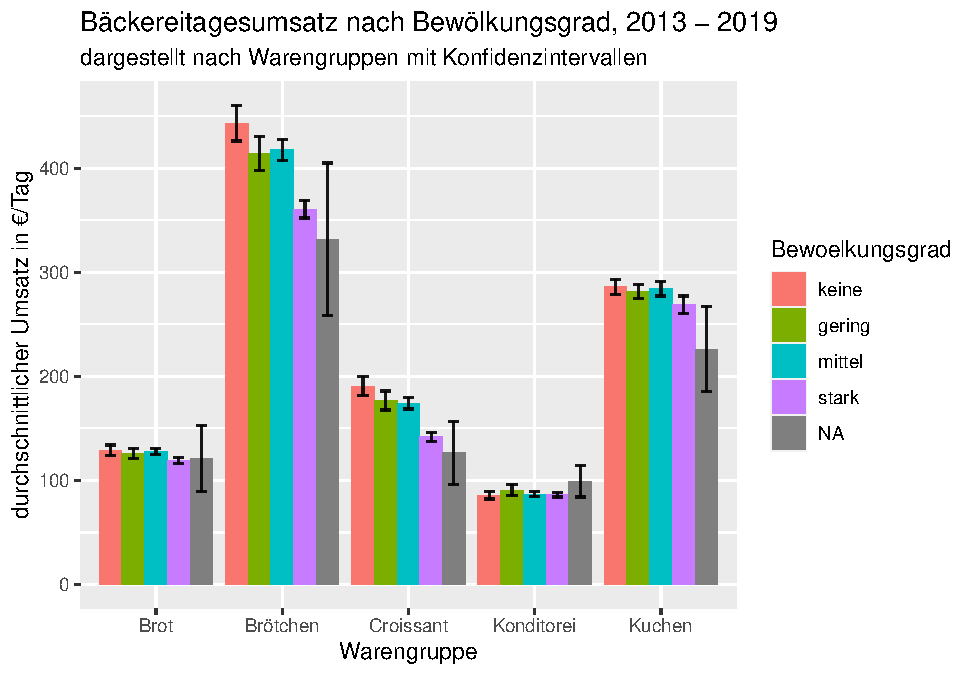
\includegraphics{Praesentation_files/figure-latex/unnamed-chunk-3-1.pdf}

\hypertarget{b.-bewuxf6lkung}{%
\paragraph{b. Bewölkung}\label{b.-bewuxf6lkung}}

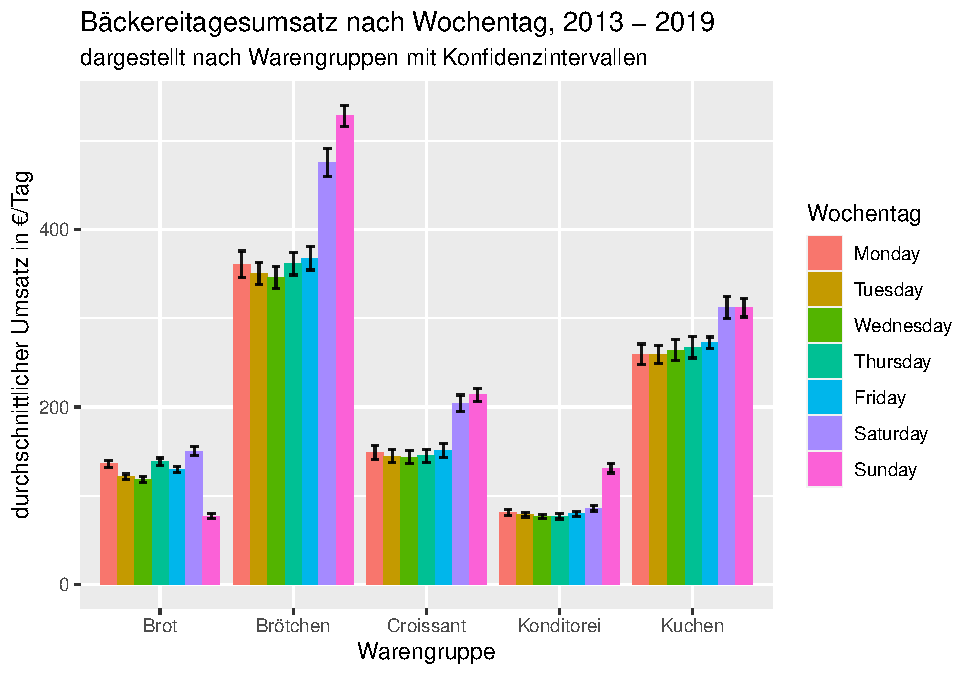
\includegraphics{Praesentation_files/figure-latex/unnamed-chunk-4-1.pdf}

\hypertarget{c.-wochentag}{%
\paragraph{c.~Wochentag}\label{c.-wochentag}}

\includegraphics{Praesentation_files/figure-latex/unnamed-chunk-5-1.pdf}

\hypertarget{optimierung-des-neuronalen-netztes}{%
\subsection{2. Optimierung des neuronalen
Netztes}\label{optimierung-des-neuronalen-netztes}}

\begin{itemize}
\tightlist
\item
  Hyperparameter:

  \begin{itemize}
  \tightlist
  \item
    Anzahl der Knoten im Hidden Layer
  \item
    Aktivierungsfunktion
  \item
    Dropout im Hidden Layer
  \item
    Learning Rate
  \end{itemize}
\item
  Datensätze:

  \begin{itemize}
  \tightlist
  \item
    Datenform von bestimmten Variablen verändert / angepasst
  \item
    Erstellung synthetischer Daten
  \end{itemize}
\end{itemize}

\hypertarget{hyperparameter}{%
\subsubsection{Hyperparameter}\label{hyperparameter}}

\hypertarget{a.-aufstellung-des-modells}{%
\paragraph{a. Aufstellung des
Modells}\label{a.-aufstellung-des-modells}}

\begin{Shaded}
\begin{Highlighting}[]

\NormalTok{model }\OperatorTok{=}\NormalTok{ Sequential([}
\NormalTok{  InputLayer(input\_shape }\OperatorTok{=}\NormalTok{ (}\BuiltInTok{len}\NormalTok{(r.training\_features.keys()), )),}
\NormalTok{  BatchNormalization(),}
\NormalTok{  Dense(}\BuiltInTok{len}\NormalTok{(r.training\_features.keys()), activation }\OperatorTok{=} \StringTok{\textquotesingle{}swish\textquotesingle{}}\NormalTok{),}
\NormalTok{  Dropout(}\FloatTok{0.2}\NormalTok{),}
\NormalTok{  Dense(}\BuiltInTok{len}\NormalTok{(r.training\_features.keys()), activation }\OperatorTok{=} \StringTok{\textquotesingle{}swish\textquotesingle{}}\NormalTok{),}
\NormalTok{  Dropout(}\FloatTok{0.2}\NormalTok{),}
\NormalTok{  Dense(}\BuiltInTok{len}\NormalTok{(r.training\_features.keys()), activation }\OperatorTok{=} \StringTok{\textquotesingle{}swish\textquotesingle{}}\NormalTok{),}
\NormalTok{  Dense(}\DecValTok{5}\NormalTok{)}
\NormalTok{])}
\end{Highlighting}
\end{Shaded}

\hypertarget{b.-schuxe4tzung-des-neuronalen-netzes}{%
\paragraph{b. Schätzung des neuronalen
Netzes}\label{b.-schuxe4tzung-des-neuronalen-netzes}}

\begin{Shaded}
\begin{Highlighting}[]
\CommentTok{\# definition of the loss function and the optimazation function with hyperparameters}
\NormalTok{model.}\BuiltInTok{compile}\NormalTok{(loss}\OperatorTok{=}\StringTok{"mape"}\NormalTok{, optimizer}\OperatorTok{=}\NormalTok{Adam(learning\_rate}\OperatorTok{=}\FloatTok{0.001}\NormalTok{))}

\CommentTok{\#Schätzung des Modells}
\NormalTok{history }\OperatorTok{=}\NormalTok{ model.fit(r.training\_features, r.training\_labels, epochs}\OperatorTok{=}\DecValTok{300}\NormalTok{,}
\NormalTok{                    validation\_data }\OperatorTok{=}\NormalTok{ (r.validation\_features, r.validation\_labels), verbose}\OperatorTok{=}\DecValTok{0}\NormalTok{)}

\NormalTok{model.save(}\StringTok{"python\_model.h5"}\NormalTok{)}
\end{Highlighting}
\end{Shaded}

\hypertarget{c.-graphische-ausgabe-der-modelloptimierung}{%
\paragraph{c.~Graphische Ausgabe der
Modelloptimierung}\label{c.-graphische-ausgabe-der-modelloptimierung}}

\includegraphics{Praesentation_files/figure-latex/unnamed-chunk-11-1.pdf}

\hypertarget{d.-grafischer-vergleich-der-vorhergesagten-tatsuxe4chlicher-preise-fuxfcr-die-trainings--und-validierungsdaten}{%
\paragraph{d.~Grafischer Vergleich der vorhergesagten \& tatsächlicher
Preise für die Trainings- und
Validierungsdaten}\label{d.-grafischer-vergleich-der-vorhergesagten-tatsuxe4chlicher-preise-fuxfcr-die-trainings--und-validierungsdaten}}

\begin{verbatim}
## 
## MAPE Warengruppe 1:  17.13
\end{verbatim}

\begin{verbatim}
## 
## MAPE Warengruppe 2:  11.21
\end{verbatim}

\begin{verbatim}
## 
## MAPE Warengruppe 3:  16.62
\end{verbatim}

\begin{verbatim}
## 
## MAPE Warengruppe 4:  20.25
\end{verbatim}

\begin{verbatim}
## 
## MAPE Warengruppe 5:  13.05
\end{verbatim}

\begin{verbatim}
## 
## MAPE Warengruppe 1:  18.72
\end{verbatim}

\begin{verbatim}
## 
## MAPE Warengruppe 2:  11.84
\end{verbatim}

\begin{verbatim}
## 
## MAPE Warengruppe 3:  18.89
\end{verbatim}

\begin{verbatim}
## 
## MAPE Warengruppe 4:  20.22
\end{verbatim}

\begin{verbatim}
## 
## MAPE Warengruppe 5:  13.61
\end{verbatim}

\begin{verbatim}
## 
## Mean Training MAPE: 15.652
\end{verbatim}

\begin{verbatim}
## Mean Validation MAPE: 16.656
\end{verbatim}

\includegraphics{Praesentation_files/figure-latex/unnamed-chunk-12-1.pdf}
\includegraphics{Praesentation_files/figure-latex/unnamed-chunk-12-2.pdf}

\hypertarget{synthetische-daten}{%
\subsubsection{Synthetische Daten}\label{synthetische-daten}}

\hypertarget{dokumentation-des-package-synthpop}{%
\paragraph{Dokumentation des Package
``synthpop''}\label{dokumentation-des-package-synthpop}}

\includegraphics{/Users/armandocriscuolo/Desktop/Bildschirm­foto 2023-01-16 um 19.40.33.png}
Link:
\url{https://cran.r-project.org/web/packages/synthpop/synthpop.pdf}

\hypertarget{reale-daten}{%
\paragraph{Reale Daten}\label{reale-daten}}

\begin{verbatim}
##         Datum      Brot Brötchen
## 1  2013-07-01 148.82835 535.8563
## 2  2013-07-02 159.79376 546.7808
## 3  2013-07-03 111.88559 427.3433
## 4  2013-07-04 168.86494 454.8596
## 5  2013-07-05 171.28075 492.8188
## 6  2013-07-06 174.55236 631.9061
## 7  2013-07-07  92.63776 695.2557
## 8  2013-07-08 135.50024 538.5292
## 9  2013-07-09 136.04838 585.9573
## 10 2013-07-10 135.13231 567.3658
\end{verbatim}

\hypertarget{synthetische-daten-1}{%
\paragraph{Synthetische Daten}\label{synthetische-daten-1}}

\begin{verbatim}
##         Datum     Brot Brötchen
## 1  2013-07-03 174.5524 631.9061
## 2  2013-07-04 171.2808 646.7890
## 3  2013-07-04 171.2808 631.9061
## 4  2013-07-05 148.8284 535.8563
## 5  2013-07-05 148.8284 695.2557
## 6  2013-07-06 174.5524 855.6191
## 7  2013-07-07 161.2647 454.8596
## 8  2013-07-08 135.1323 567.3658
## 9  2013-07-09 101.4475 535.8563
## 10 2013-07-09 116.8214 585.9573
\end{verbatim}

\hypertarget{evaluationsergebnis-fuxfcr-den-zeitraum-09.06.---30.07.2019}{%
\subsection{3. Evaluationsergebnis für den Zeitraum 09.06. -
30.07.2019}\label{evaluationsergebnis-fuxfcr-den-zeitraum-09.06.---30.07.2019}}

\begin{verbatim}
## Rows: 255 Columns: 3
## -- Column specification --------------------------------------------------------
## Delimiter: ","
## dbl  (2): Warengruppe, Umsatz
## date (1): Datum
## 
## i Use `spec()` to retrieve the full column specification for this data.
## i Specify the column types or set `show_col_types = FALSE` to quiet this message.
\end{verbatim}

\begin{verbatim}
## Realer MAPE: 17.45
\end{verbatim}

\hypertarget{umsatzvorhersage-fuxfcr-den-09.06.2019}{%
\subsection{4. Umsatzvorhersage für den
09.06.2019}\label{umsatzvorhersage-fuxfcr-den-09.06.2019}}

\includegraphics{Praesentation_files/figure-latex/unnamed-chunk-17-1.pdf}

\end{document}
